\chapter{Hướng tiếp cận và đề xuất hệ thống}\label{chap:design}
Chương này phân tích yêu cầu, nêu các bất biến thiết kế và mô tả kiến trúc cùng thiết kế chi tiết từng thành phần: tổ chức nội dung, chính sách dạy, truy xuất, diễn đạt và kiểm chứng, bộ chấm và mô hình người học, bộ chọn nước đi bằng bandit, mở rộng sang Tiếng Anh và giọng nói, cuối cùng là dữ liệu và triển khai.

\section{Kiến trúc tổng thể}\label{sec:architecture}
Hệ thống gồm hai phần: phần dựng nội dung chạy trước khi học và phần hội thoại chạy trong mỗi lượt. Phần dựng nội dung biến tài liệu của giáo viên thành gói giáo án có cấu trúc: hệ thống đọc từng trang PDF bằng lớp chữ và nhận dạng ký tự, cắt câu hỏi và đáp án bằng bộ phân tích tất định, trích nội dung từng tiết kèm kiểm đáp án bằng cách tính lại từ đề, rồi dựng đồ thị tri thức gồm $19$ tiết và $28$ quan hệ (mục~\ref{sec:content-design}). Phần còn thiếu của tài liệu, như gợi ý ở bậc thấp hay ý chính của bài, do mô hình ngôn ngữ soạn nháp và chỉ được dùng sau khi qua kiểm chứng và được giáo viên duyệt. Nội dung cũng được cắt thành đoạn, lập chỉ mục từ khóa và vector để phục vụ truy xuất.

Hình~\ref{fig:architecture} trình bày toàn bộ kiến trúc với ba vùng. Vùng trên dựng đồ thị tri thức từ tài liệu của giáo viên. Vùng giữa là một lượt dạy: bộ điều phối, chính sách Socratic, bộ chấm, sổ sự kiện và mô hình người học đều tất định, còn mô hình ngôn ngữ chỉ diễn đạt nước đi và câu mẫu, và lời của nó chỉ đến học sinh khi qua bộ kiểm chứng. Vùng dưới dựng chỉ mục truy xuất lai từ kho học liệu.

\begin{figure}[H]
\centering
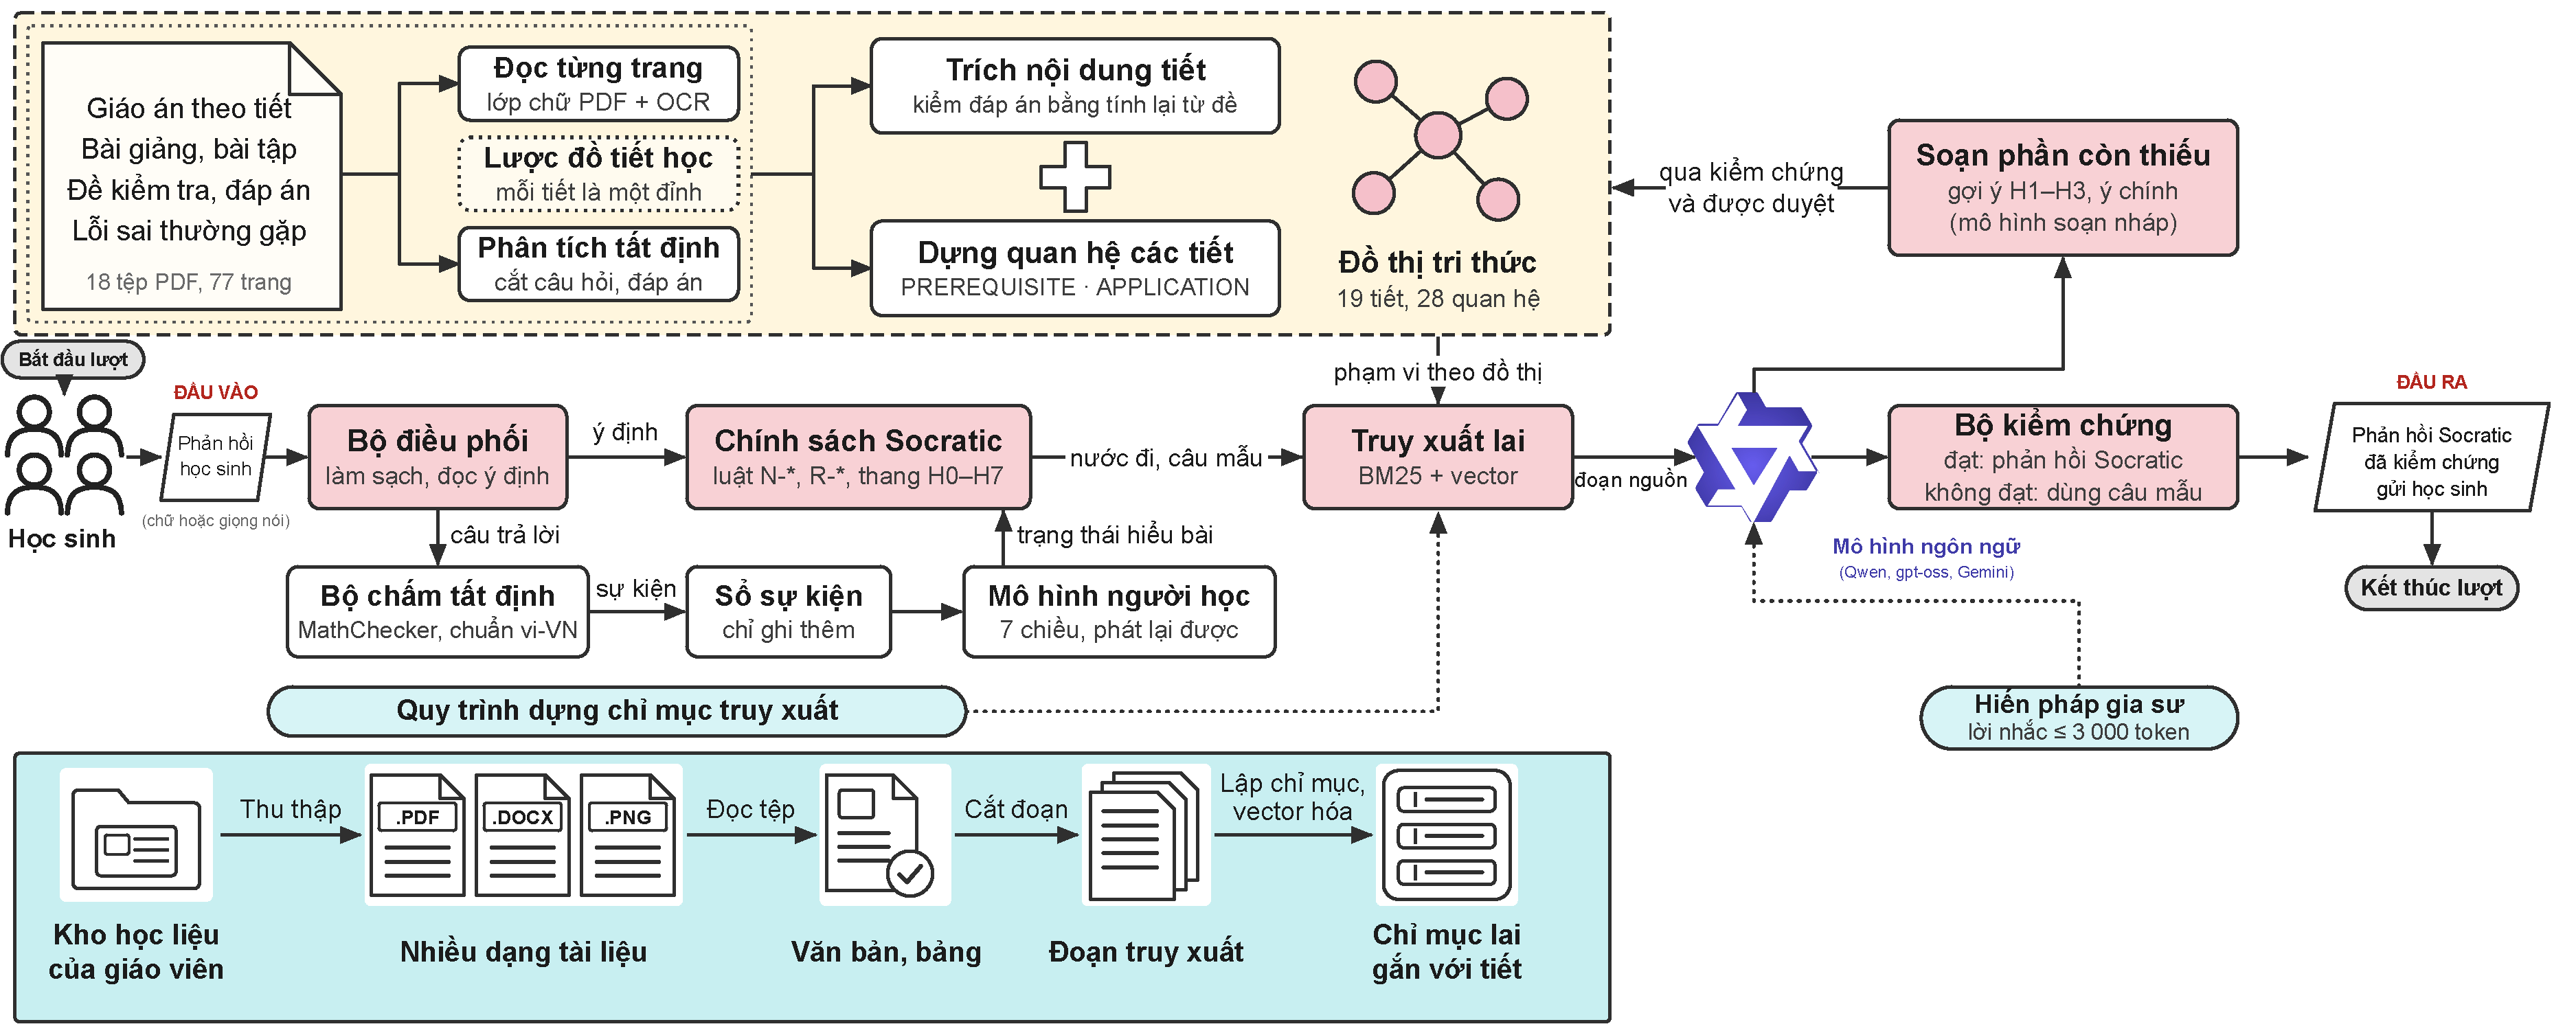
\includegraphics[width=\linewidth]{figures/fig-architecture.pdf}
\caption{Kiến trúc tổng thể của CAVAT. Đầu vào của một lượt là phản hồi của học sinh (chữ hoặc giọng nói), đầu ra là phản hồi đã qua bộ kiểm chứng gửi lại học sinh; hai vùng ở trên và dưới là các quy trình chạy trước, nhận tài liệu của giáo viên và cho ra đồ thị tri thức và chỉ mục truy xuất. Biểu tượng mô hình ngôn ngữ đại diện cho chuỗi mô hình do cổng AI điều phối (gpt-oss-120b, Qwen, gpt-oss-20b, Gemini), và bộ chọn nước đi bằng bandit (mục~\ref{sec:bandit-design}) nằm trong khối chính sách Socratic.}
\label{fig:architecture}
\end{figure}

Trong vùng giữa, mỗi lượt được xử lý theo một chuỗi cố định (Hình~\ref{fig:turn-flow}). Bộ đọc nhận phản hồi của học sinh, nhận ý định và chuyển câu trả lời cho bộ chấm. Chính sách chọn nước đi và bậc gợi ý theo trạng thái câu hỏi và mức hiểu bài. Mô hình ngôn ngữ nhận nước đi, câu mẫu và đoạn nguồn trong một lời nhắc không quá $3\,000$ token rồi soạn lời nháp cho Gia sư AI. Bộ kiểm chứng đánh giá lời nháp: lời đạt được gửi cho học sinh, lời không đạt bị thay bằng câu mẫu đã duyệt. Mọi bước ghi sự kiện vào sổ chỉ ghi thêm, và phép chiếu mức hiểu đọc sổ này để cung cấp trạng thái hiểu bài cho lượt sau. Mô hình ngôn ngữ vì vậy là thành phần duy nhất không tất định, và nó không quyết định nước đi, không chấm điểm, không ghi mức hiểu.

\begin{figure}[H]
\centering
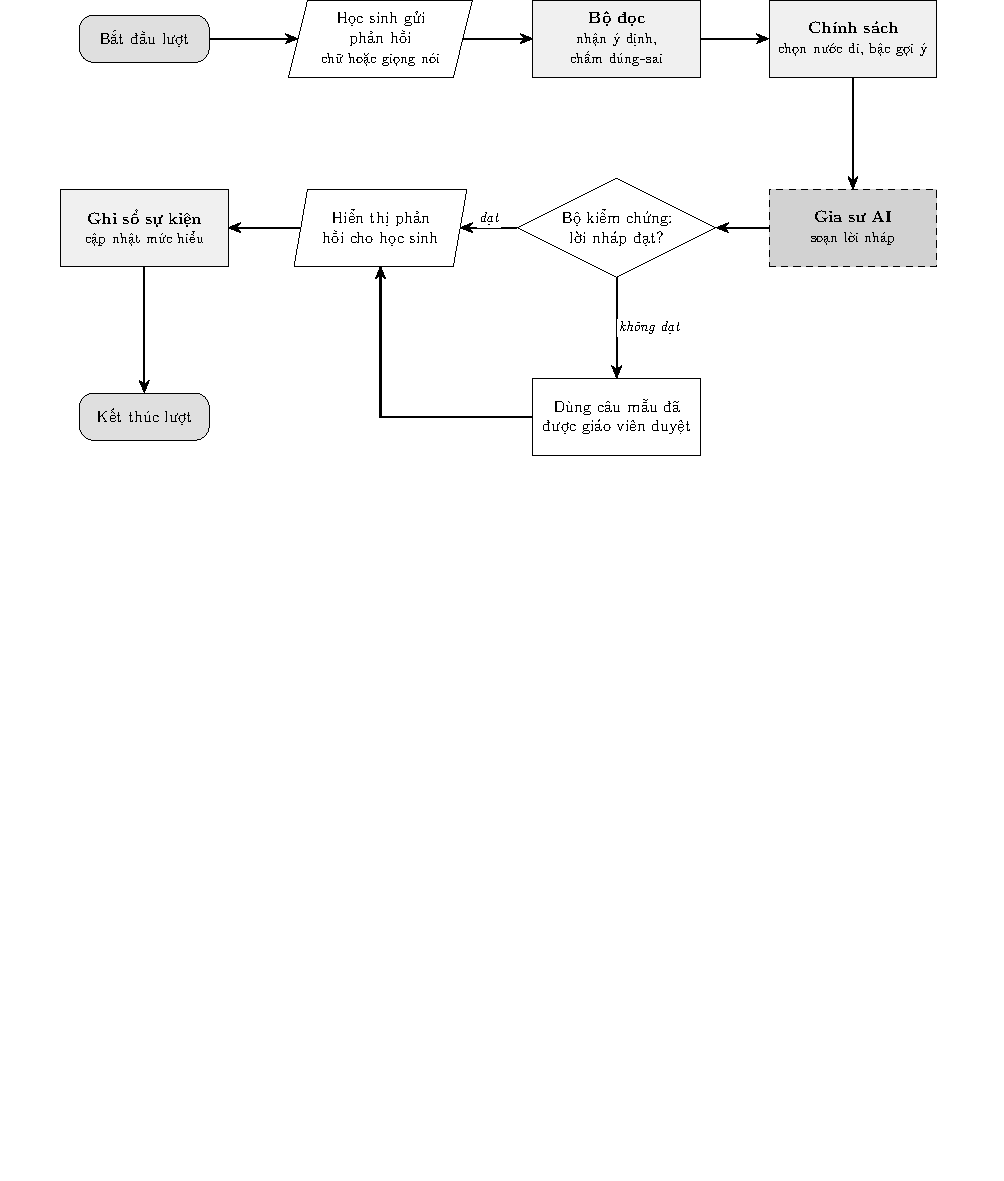
\includegraphics{figures/pdf/fig-turn-flow.pdf}
\caption{Luồng xử lý một lượt dạy. Hình bầu dục: bắt đầu và kết thúc; hình bình hành: dữ liệu vào và ra; hình thoi: điều kiện; hình chữ nhật xám nhạt: thành phần tất định; hình chữ nhật xám đậm nét đứt: thành phần duy nhất dùng mô hình ngôn ngữ.}
\label{fig:turn-flow}
\end{figure}

\section{Yêu cầu và các bất biến thiết kế}\label{sec:nfr}

\subsection{Yêu cầu}
Hệ thống phục vụ ba loại người dùng: giáo viên cung cấp tài liệu, duyệt nội dung và xem báo cáo; học sinh học bằng văn bản hoặc giọng nói trên trang web dùng được cả ở điện thoại; phụ huynh xem tiến bộ qua tài khoản của con. Từ đó hệ thống có sáu chức năng: tạo gói giáo án từ tài liệu giáo viên và chỉ dùng nội dung đã duyệt; dạy từng bài theo vòng có thứ tự trên đồ thị tri thức, trong đó bài tập chỉ là một bước; tương tác theo phương pháp Socratic; chấm câu trả lời theo cách viết của trẻ em Việt Nam; ước lượng mức hiểu từ kết quả học; và trình bày kết quả qua ba trang báo cáo riêng. Phạm vi khóa ở hai chương Toán lớp 5 và một đơn vị Tiếng Anh lớp 5 (Unit~11), để mọi thành phần được kiểm chứng kỹ trên lượng nội dung nhỏ và để chủ dự án, vốn là giáo viên, duyệt được toàn bộ nội dung sư phạm.

Các yêu cầu phi chức năng xuất phát từ hai ràng buộc: hệ thống dùng dịch vụ miễn phí nên hạn mức là ràng buộc thiết kế, và người học là trẻ em nên lỗi nội dung không được phép đi qua. Về hạn mức, lời nhắc không quá $3\,000$ token vì hạn mức $8\,000$ token mỗi phút, mỗi buổi và mỗi chương có trần số lệnh gọi mô hình, và mỗi nước đi có câu mẫu đã duyệt để buổi học không dừng khi nhà cung cấp lỗi. Về tái lập và kiểm toán, cùng một sổ sự kiện luôn cho cùng quyết định và cùng điểm, mỗi quyết định ghi mã luật và mỗi lệnh gọi mô hình ghi vào sổ. Về dữ liệu, mọi tài liệu người học mang mã trường và mọi truy vấn lọc theo mã đó vì MongoDB không có cô lập theo hàng; trạng thái và sự kiện của một buổi nằm trong một tài liệu ghi nguyên tử vì gói miễn phí không có giao dịch nhiều tài liệu; chỉ gửi ra ngoài dữ liệu tối thiểu (tên gọi, không họ); database kiểm thử, demo và dữ liệu thật tách hẳn nhau.

\subsection{Sáu bất biến thiết kế}
Từ các rủi ro ở Chương~\ref{chap:intro}, đồ án rút ra sáu bất biến mà hệ thống phải giữ bất kể mô hình ngôn ngữ nói gì. Bảng~\ref{tab:invariants} cho biết từng bất biến do thành phần nào bảo đảm, thuộc loại nào và được kiểm chứng ra sao. Hai loại bảo đảm khác nhau về bản chất. Bảo đảm \emph{theo cấu trúc} nghĩa là vi phạm là không thể, vì thành phần liên quan không có đường tới dữ liệu cấm: bộ dựng lời nhắc không có đáp án câu kiểm tra thì mô hình không thể nói ra đáp án đó từ ngữ cảnh. Bảo đảm \emph{kiểm sau khi sinh} nghĩa là mô hình có thể sinh lỗi nhưng bộ kiểm chứng chặn được, nên chỉ đúng ở mức bộ kiểm bắt được lỗi. Hai loại không có cùng độ chắc chắn, và Chương~\ref{chap:eval} báo cáo riêng từng loại.

Bộ kiểm chứng sau khi sinh rà bốn lỗi: lộ đáp án, nhiều hơn một câu hỏi, quá dài, và số hoặc thuật ngữ không có nguồn. Lỗi lộ đáp án bảo vệ B1 ở đầu ra, lỗi không có nguồn bảo vệ B6, còn hai lỗi kia là quy tắc diễn đạt chứ không thuộc bất biến nào. Các bất biến B2 đến B5 do cấu trúc bảo đảm nên không cần bộ kiểm.

\begin{table}[H]
\centering
\caption{Sáu bất biến thiết kế, thành phần bảo đảm và cách kiểm chứng}\label{tab:invariants}
\small
\begin{tabular}{>{\raggedright\arraybackslash}p{3.6cm}>{\raggedright\arraybackslash}p{3.7cm}>{\raggedright\arraybackslash}p{2.1cm}>{\raggedright\arraybackslash}p{3.7cm}}
\toprule
Bất biến & Thành phần và cơ chế & Loại bảo đảm & Kiểm chứng (mục) \\
\midrule
B1. Đáp án câu kiểm tra không có trong ngữ cảnh gửi mô hình & Bộ dựng lời nhắc không đưa đáp án; kiểm tra chặn gợi ý ở bậc H1 & Cấu trúc, cộng kiểm sau sinh & Luật tất định trên lời nháp: số lượt chứa đáp án (\ref{sec:eval-socratic}) \\
B2. Chính sách tất định chọn nước đi, mô hình chỉ diễn đạt & Hàm quyết định có phiên bản, mô hình chỉ được gọi cho một tập nước đi & Cấu trúc & So với lời nhắc Socratic có và không có bộ lọc (\ref{sec:eval-socratic}); chưa tách riêng được khỏi bộ lọc \\
B3. Đúng sai Toán do bộ chấm tất định & Bộ chấm theo chuẩn viết số Việt Nam, không gọi mô hình & Cấu trúc & Độ đúng trên câu trả lời gán nhãn tay (\ref{sec:eval-grading}) \\
B4. Mức hiểu là phép chiếu từ sổ sự kiện & Hàm gấp thuần túy; nhãn của mô hình chỉ là bằng chứng có trọng số & Cấu trúc & Phát lại $2\times500$ chuỗi, so với công thức viết thẳng (\ref{sec:eval-learner}) \\
B5. Không dạy trước nội dung bài sau & Phạm vi truy xuất chỉ gồm bài đang học và tổ tiên trên đồ thị & Cấu trúc & Số đoạn bài sau trong kết quả đầu (\ref{sec:eval-rag}) \\
B6. Mọi khẳng định có căn cứ & Kiểm số, thuật ngữ và từ so với nguồn; thử lại rồi dùng câu mẫu & Kiểm sau sinh & Số lời nháp lỗi bị chặn (\ref{sec:eval-model}) \\
\bottomrule
\end{tabular}
\end{table}

Hai nguyên tắc kỹ thuật đi kèm: ràng buộc của buổi học được thực thi ở máy chủ chứ không chỉ ẩn nút ở giao diện, và máy khách không bao giờ được chọn mô hình. Ngoài sáu bất biến, khi thêm môn Tiếng Anh thì hành vi, công thức, ngưỡng và lời nhắc của Toán không được đổi (mục~\ref{sec:english-design}), còn lời nhắc, chính sách và chính sách mức hiểu đều là hiện vật có phiên bản và mọi thay đổi chúng đòi chạy lại bộ đánh giá hồi quy. Công thức và ngưỡng không có trong khung đánh giá gốc được đánh dấu là diễn giải khai báo (DI), để người đọc phân biệt điều có nguồn với lựa chọn của đồ án.

\section{Tổ chức nội dung: gói giáo án và đồ thị tri thức}\label{sec:content-design}
Một chương được biểu diễn bằng đồ thị có hướng $G=(V,E)$. Mỗi đỉnh là một bài học, mỗi cạnh $(u,v)$ mang một trong hai kiểu: tiên quyết (học $u$ trước $v$) hoặc vận dụng ($v$ vận dụng $u$). Hai chương Toán có $19$ bài và $28$ cạnh: chương Số thập phân có $11$ bài và $17$ cạnh, chương Diện tích có $8$ bài và $11$ cạnh; Unit~11 Tiếng Anh có $6$ bài. Mỗi đỉnh đi kèm một gói nội dung gồm các cách giảng lý thuyết, phương pháp làm bài, ví dụ mẫu, ghi chú lỗi sai thường gặp, ngân hàng câu hỏi và các ý chính của bài để học sinh kể lại. Một câu hỏi có đề bài và đặc tả đáp án (số, trắc nghiệm, so sánh, sắp xếp, đúng sai hoặc mở), mức nhận thức (A đến E và chẩn đoán), độ khó từ $0$ đến $1$, mục đích (kiểm tra hiểu, luyện tập, kiểm tra cuối bài, ôn tập) và thang gợi ý riêng. Mức nhận thức và độ khó quyết định chiều của mô hình người học mà câu trả lời cung cấp bằng chứng (mục~\ref{sec:learner-design}).

Gói giáo án được dựng từ $18$ tài liệu thật của giáo viên ($77$ trang: giáo án, sách giáo khoa, sách bài tập, phiếu bài tập), không soạn tay. Ba luồng chạy song song trên văn bản đã đọc: dựng lược đồ bài học, cắt từng câu hỏi và đáp án, và trích nội dung từng bài. Mọi đáp án trích được đều được kiểm lại bằng cách tính lại từ đề; đáp án mâu thuẫn với đề bị loại và được liệt kê trong báo cáo thay vì được dạy. Ngân hàng của chương Số thập phân có $234$ câu ($46$ câu kiểm tra), của chương Diện tích có $155$ câu ($33$ câu kiểm tra). Phần tài liệu còn thiếu được mô hình soạn nháp, chỉ dùng sau khi qua kiểm chứng và được giáo viên duyệt, và nội dung của giáo viên luôn thắng nội dung do mô hình đề xuất. Quyết định duyệt gắn với phiên bản xuất bản của kế hoạch, nên mỗi buổi học dùng đúng phiên bản chương lúc bắt đầu và một buổi cũ phát lại luôn cho cùng kết quả.

Cùng nội dung được cắt thành các đoạn truy xuất. Chỉ mục xuất bản của hai chương Toán có $221$ đoạn: $83$ đoạn trích từ tài liệu nguồn, $38$ đoạn lý thuyết, $27$ ví dụ mẫu, $19$ đoạn phương pháp và $54$ ghi chú lỗi quan niệm. Mỗi đoạn mang mã bài của nó trong đồ thị, nên truy xuất biết câu hỏi được đặt khi học sinh đang ở bài nào và biết khoảng cách trên đồ thị đến bài chứa đoạn (mục~\ref{sec:retrieval-design}).

\section{Chính sách dạy: vòng sáu bước và thang gợi ý}\label{sec:policy-design}
Chính sách dạy có hai tầng, cả hai tất định. Tầng trên chọn bài và hoạt động trên đồ thị tri thức theo vòng sáu bước. Tầng dưới điều khiển một câu hỏi từ lúc nêu đến lúc khép, chọn nước đi và bậc gợi ý ở từng lượt. Phần diễn đạt thành lời thuộc về mô hình ngôn ngữ và là phần duy nhất không tất định (mục~\ref{sec:render-design}). Mỗi luật của chính sách có một mã tra cứu trong mã nguồn (dạng \rid{N-*} cho tầng trên và \rid{R-*} cho tầng dưới); mã chỉ để truy vết quyết định và được ghi kèm mỗi quyết định.

\subsection{Vòng sáu bước trên đồ thị}
Gia sư dạy mỗi bài theo sáu bước (Hình~\ref{fig:teaching-loop}). Bước một ôn bài tiên quyết rồi giảng lý thuyết của bài mới, vì học sinh cần nhớ điều đã học trước khi nghe điều mới. Bước hai kiểm tra hiểu bằng một câu hỏi và việc mời học sinh kể lại ý chính. Bước ba đưa ví dụ mẫu rồi một câu cùng làm, trong đó gia sư và học sinh giải chung. Bước bốn luyện tập với độ khó tăng dần, bước năm vận dụng vào tình huống mới, và bước sáu quyết định bài đã qua chưa. Vòng sáu bước là cách đếm của chủ dự án từ ngày 09/11/2026, thay vòng bảy bước trước đó mà không đổi luật điều khiển, giáo án hay công thức mức hiểu; buổi học đã lưu theo vòng cũ vẫn hiển thị đúng nhờ một bảng chuyển.

\begin{figure}[H]
\centering
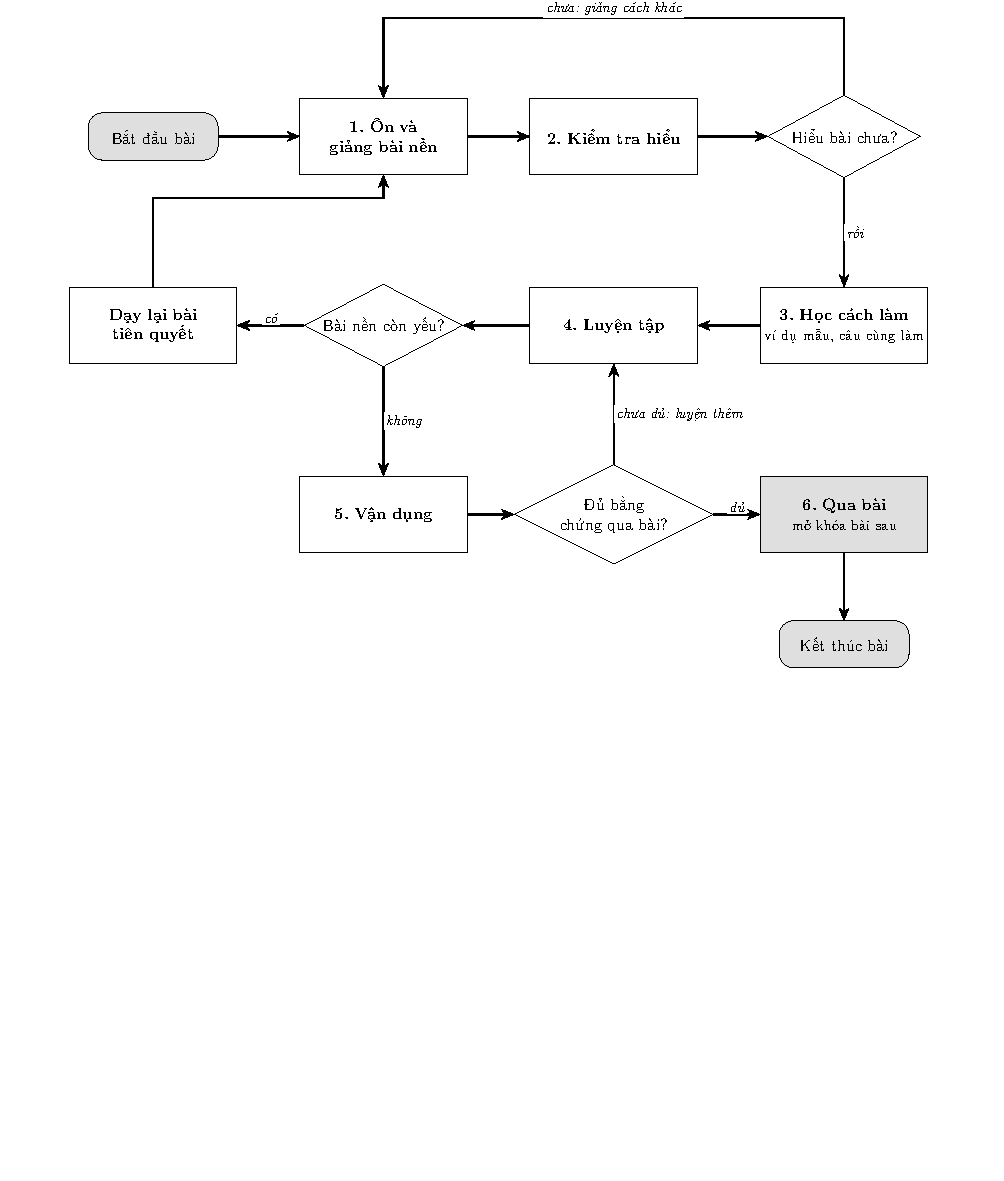
\includegraphics{figures/pdf/fig-teaching-loop.pdf}
\caption{Vòng sáu bước dạy một bài. Hình thoi là các điều kiện do luật của chính sách quyết định; học sinh chưa hiểu thì được giảng cách khác, bài nền còn yếu thì dạy lại bài tiên quyết trước, chưa đủ bằng chứng thì luyện thêm.}
\label{fig:teaching-loop}
\end{figure}

Mười bốn luật tầng trên chạy theo thứ tự ưu tiên và luật đầu tiên có điều kiện thỏa quyết định hành động kế tiếp. Chúng đọc trực tiếp phép chiếu mức hiểu ở mục~\ref{sec:learner-design}. Gia sư tạm dừng bài hiện tại để dạy lại bài tiên quyết khi một lỗi nghiêm trọng thuộc bài tiên quyết, hoặc khi hai lần kiểm tra không qua trong lúc bài tiên quyết còn yếu. Gia sư cho một câu khởi động của bài trước khi vào bài mới mà bài trước chưa có bằng chứng trong buổi, và xen một câu của bài đã qua để ôn lại. Bài được tính là qua khi thỏa quy tắc qua bài (mục~\ref{sec:learner-design}); hết ngân sách câu mà chưa qua thì bài được ghi là cần học lại.

\subsection{Thang gợi ý từ H0 đến H7}
Trong một câu hỏi, sự trợ giúp được lượng hóa bằng thang tám bậc từ H0 (không gợi ý) đến H7 (giải thích đầy đủ), theo hai trục: bậc là bao nhiêu trợ giúp, mục tiêu là trợ giúp nhắm vào đâu (đề bài, khái niệm, chiến lược, bước làm, cách viết đáp số hoặc việc tự kiểm tra). Bảng~\ref{tab:ladder} nêu tám bậc với ví dụ cho câu ``viết phân số $9/10$ dưới dạng số thập phân'' (đáp án $0{,}9$). Mỗi bậc có một trọng số độc lập $\iota_h$ do khung đánh giá quy định, được mô hình người học dùng ở mục~\ref{sec:learner-design}, nên gia sư và bộ đánh giá nói cùng một ngôn ngữ về mức học sinh đã được giúp.

\begin{table}[H]
\centering
\caption{Thang gợi ý. Trọng số $\iota_3$ và $\iota_5$ là diễn giải khai báo (DI) nội suy giữa các giá trị của khung đánh giá.}\label{tab:ladder}
\small
\begin{tabular}{>{\raggedright\arraybackslash}p{0.9cm}>{\raggedright\arraybackslash}p{2.9cm}>{\raggedright\arraybackslash}p{8.4cm}r}
\toprule
Bậc & Tên & Ví dụ & $\iota_h$ \\
\midrule
H0 & không gợi ý & --- & $1{,}00$ \\
H1 & câu hỏi định hướng & ``Mình cần viết $9/10$ thành số thập phân. Con đọc phân số này giúp cô nhé?'' & $0{,}85$ \\
H2 & nhắc khái niệm & ``Mẫu số 10 cho biết phần thập phân có mấy chữ số?'' & $0{,}70$ \\
H3 & gợi ý chiến lược & ``Con thử viết chữ số 9 vào hàng phần mười xem sao?'' & $0{,}60$ \\
H4 & cho một bước trung gian & ``Phần nguyên là 0, hàng phần mười là chữ số 9. Vậy viết thế nào?'' & $0{,}50$ \\
H5 & chia nhỏ bài & ``Mình làm từng bước nhỏ. Mẫu số của $9/10$ là bao nhiêu?'' & $0{,}35$ \\
H6 & cùng làm từng bước & Trình bày các bước, học sinh làm bước cuối & $0{,}20$ \\
H7 & giải thích đầy đủ & Giải thích như lời giải mẫu rồi mời trình bày lại & $0{,}00$ \\
\bottomrule
\end{tabular}
\end{table}

Mỗi câu luyện tập mang thang gợi ý riêng: các bậc H1 đến H3 do giáo viên duyệt, các bậc cao hơn rút từ lời giải, và khi câu thiếu một bậc thì gợi ý chung của bài thay vào. Thang không bao giờ tự nói đáp án; chỉ bậc H7 được phép nói đáp án và chỉ ở hoạt động luyện tập. Trong bài kiểm tra, bậc gợi ý bị chặn ở H1 và câu vượt trần được khép với trạng thái chưa giải được.

\subsection{Chính sách của vòng một câu hỏi}
Vòng một câu hỏi là một máy trạng thái chạy từ lúc nêu câu đến khi khép câu. Mỗi tin nhắn của học sinh được bộ đọc phân loại thành lần thử có thể chấm, xin gợi ý, đòi đáp án, hỏi lại đề, hỏi nghĩa một từ, lạc đề hoặc cảm xúc tiêu cực, rồi hợp vào trạng thái của câu và đưa cho hàm quyết định. Hàm này là danh sách luật có thứ tự: luật đầu tiên thỏa điều kiện quyết định nước đi, bậc và mục tiêu, và mã luật được ghi vào sổ cùng quyết định, nên mỗi hành vi của gia sư giải thích và kiểm thử được theo từng luật. Phiên bản hiện hành có $29$ luật; Bảng~\ref{tab:rules} nêu các họ chính.

{\small
\begin{longtable}{>{\raggedright\arraybackslash}p{3.3cm}>{\raggedright\arraybackslash}p{5.4cm}>{\raggedright\arraybackslash}p{6.0cm}}
\caption{Các họ luật chính của vòng một câu hỏi.}\label{tab:rules}\\
\toprule
Luật & Điều kiện & Quyết định \\
\midrule
\endfirsthead
\toprule
Luật & Điều kiện & Quyết định \\
\midrule
\endhead
\bottomrule
\endfoot
\rid{R-FIRST-WRONG} & Câu sai đầu tiên, chưa có gợi ý & Hỏi ``con đã làm thế nào''; chưa gợi ý \\
\rid{R-SLIP} & Lỗi tính toán, phương pháp đúng & Gợi ý H1, mục tiêu tự kiểm tra \\
\rid{R-MISC-HIGH} & Nhận ra lỗi quan niệm với độ tin cậy từ $0{,}7$ & Gợi ý từ H2 về khái niệm; đưa phản ví dụ khi có \\
\rid{R-LADDER}, \rid{R-ESCALATE} & Sai các lần sau; sai lặp lại cùng mục tiêu & Bậc không thấp hơn bậc đã dùng; thêm một bậc, hai bậc khi có dấu hiệu nản \\
\rid{R-DEESCALATE} & Một bước đúng sau gợi ý & Hạ một bậc, giảm dần giàn giáo \\
\rid{R-HELP-REQUEST} & Xin gợi ý, ``con không biết'', đòi đáp án & Đề nghị chọn một lần, rồi gợi ý kế tiếp; đòi đáp án thì từ chối nhẹ và gợi ý \\
\rid{R-OFF-TOPIC}, \rid{R-CLARIFY}, \rid{R-AFFECT} & Lạc đề; ``là sao ạ''; ``chán quá'' & Kéo về câu; nói lại đề; công nhận cảm xúc rồi gợi ý. Không tính là sai \\
\rid{R-FRUSTRATION}, \rid{R-FULL} & Ba lượt không tiến bộ hoặc quá $300$ giây; cùng làm vẫn không tiến & Cùng làm từng bước (H6); giải thích đầy đủ (H7, chỉ khi luyện tập), rồi mời giảng lại \\
\rid{R-VERIFY} & Trả lời đúng và thuộc diện cần xác nhận (DI) & Hỏi ``vì sao'' \\
\rid{R-ASSESS-CAP} & Câu của bài kiểm tra & Bậc tối đa H1; quá thì khép câu \\
\end{longtable}}

Chính sách không dùng số ngẫu nhiên: việc chọn câu đúng nào để hỏi ``vì sao'' dùng giá trị băm của mã câu, nên cùng một buổi học luôn cho cùng một quyết định và phát lại được. Những lượt không phải một lần thử, như lạc đề hay ``là sao ạ'', không bị tính là sai vì chấm một lời than thở là sai sẽ phạt học sinh vì điều em không làm. Câu đúng từng phần không làm tăng bậc gợi ý, và câu đúng sau giải thích đầy đủ không bao giờ được tính là thành công của bài.

\section{Truy xuất lai theo đồ thị tri thức}\label{sec:retrieval-design}
Truy xuất trong dạy học phục vụ bốn việc: chọn nội dung giảng tiếp theo, tìm căn cứ cho gợi ý, trả lời câu hỏi do học sinh đặt ra và giải thích một khái niệm. Cả bốn chịu hai ràng buộc mà truy xuất tổng quát không có. Ràng buộc phạm vi cấm dùng đoạn của bài chưa học để phản hồi, nhằm tránh dạy trước. Ràng buộc nền tảng chuyển những câu hỏi không có đoạn nguồn phù hợp cho giáo viên thay vì tạo thông tin không căn cứ. Hình~\ref{fig:retrieval-flow} tóm tắt luồng truy xuất.

\begin{figure}[H]
\centering
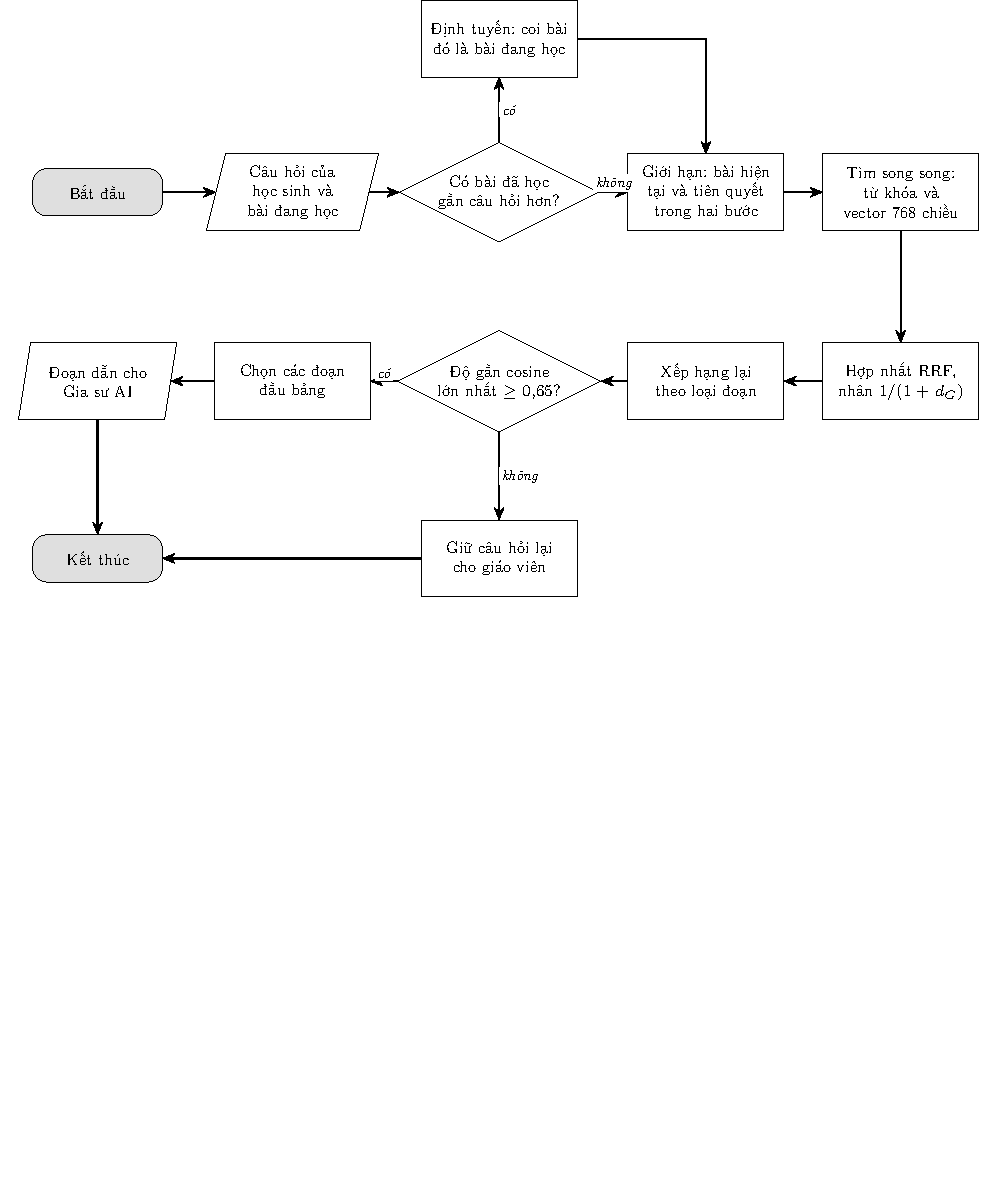
\includegraphics[width=\linewidth]{figures/pdf/fig-retrieval-flow.pdf}
\caption{Luồng truy xuất lai. Có hai cơ chế riêng của dạy học: định tuyến theo chủ đề (hình thoi đầu) và bước kiểm tra căn cứ (hình thoi sau, ngưỡng cosine $0{,}65$).}
\label{fig:retrieval-flow}
\end{figure}

\subsection{Phạm vi, từ khóa, ngữ nghĩa và hợp nhất}
Bước đầu giới hạn các đoạn được xét: phạm vi gồm bài học sinh đang học và các bài tiên quyết của nó cách không quá hai bước trên đồ thị, và một đoạn thuộc nhiều bài chỉ được xét khi mọi bài của nó nằm trong phạm vi. Bài sau bài đang học nằm ngoài phạm vi, nên câu trả lời không bao giờ dựa vào nội dung chưa dạy. Mỗi đoạn mang khoảng cách $d_G$ trên đồ thị từ bài đang học đến bài chứa nó.

Hai bộ xếp hạng chạy song song trong phạm vi. BM25 theo từ khóa chạy trên cả dạng có dấu và dạng bỏ dấu, dùng âm tiết và cặp âm tiết liền kề làm đơn vị vì tiếng Việt viết tách âm tiết và trẻ hay gõ không dấu. Bộ so khớp ngữ nghĩa dùng độ gần cosine giữa vector câu hỏi và vector $768$ chiều của đoạn do mô hình \texttt{gemini-embedding-001} tạo. Hai danh sách được hợp nhất bằng RRF (công thức~\eqref{eq:rrf}) rồi nhân với hệ số khoảng cách đồ thị:
\begin{equation}
\mathrm{fuse}(c)=\frac{1}{1+d_G(v,\nu(c))}\sum_{r\in\{\mathrm{BM25},\,\cos\}}\frac{1}{60+\mathrm{rank}_r(c)},
\label{eq:fuse}
\end{equation}
với $v$ là bài đang học và $\nu(c)$ là bài chứa đoạn $c$.

\subsection{Xếp hạng lại theo sư phạm}
Danh sách hợp nhất được xếp hạng lại: $\mathrm{score}(c)=\mathrm{fuse}(c)\,\kappa_m(\text{loại}_c)\,\gamma(c)$. Hệ số $\kappa_m\in[0{,}8;\,1{,}5]$ ưu tiên loại đoạn theo việc truy xuất đang phục vụ (khi giảng giải: lý thuyết $1{,}5$, ví dụ mẫu $1{,}1$, phương pháp $1{,}0$; khi gợi ý: phương pháp $1{,}4$, ví dụ mẫu $1{,}3$). Hệ số $\gamma$ theo ngữ cảnh bằng $1{,}5$ cho ghi chú lỗi sai vừa nhận diện, $1{,}6$ cho đoạn định nghĩa thuật ngữ được hỏi và $1$ trong các trường hợp còn lại; các đoạn đã dùng trong buổi bị hạ điểm để gia sư không lặp một cách giảng. Các hệ số này do người phát triển chọn thủ công theo nhu cầu của từng chế độ, không tinh chỉnh trên tập đánh giá và là diễn giải khai báo; mục~\ref{sec:eval-rag} đo độ nhạy của chúng và cho thấy việc đổi hệ số chưa làm đổi kết quả, nên các hệ số chưa được biện minh bằng dữ liệu. Cuối cùng hệ thống chọn các đoạn đứng đầu trong một ngân sách ký tự cố định, kèm vết các tín hiệu của từng đoạn để giáo viên xem được lý do một đoạn được chọn.

\subsection{Định tuyến theo chủ đề}
Phạm vi theo đồ thị có một hạn chế: học sinh thường hỏi lại khái niệm của bài trước khi đang học bài mới, và hệ số $1/(1+d_G)$ đẩy đoạn của bài hiện tại lên trước đoạn thật sự trả lời. Định tuyến theo chủ đề sửa điều này. Hệ thống so khớp câu hỏi với từng bài trong phạm vi bằng độ gần cosine lớn nhất; khi một bài trước gần câu hỏi hơn bài đang học quá một lề $\varepsilon=0{,}02$, các đoạn của bài đó được coi như có $d_G=0$. Định tuyến chỉ chọn bài tiên quyết đã học, nên không phá bất biến không dạy trước. Mục~\ref{sec:eval-rag} đo tác dụng của cơ chế này: bỏ định tuyến là điều làm mức truy xuất giảm nhiều nhất.

\subsection{Kiểm tra căn cứ và tra cứu ngoài kho}
Trước khi trả lời bằng nội dung của chương, hệ thống kiểm câu hỏi có căn cứ trong kho hay không. Câu được coi là có căn cứ khi độ gần cosine lớn nhất giữa câu hỏi và các đoạn chọn được đạt ngưỡng $0{,}65$, một diễn giải khai báo của đồ án. Câu nêu thuật ngữ Toán lớp 5 mà kho không dùng, như ``hình tròn'' hay ``thể tích'', bị coi là ngoài chương dù cosine vượt ngưỡng. Câu không có căn cứ được giữ lại cho giáo viên và gia sư kéo học sinh về câu đang làm.

Khi kho không có đoạn trả lời mà câu hỏi vẫn thuộc khái niệm của bài hiện tại hay nền trực tiếp của nó, hệ thống có thể tra một ấn phẩm công khai đã xác minh của nhà xuất bản giáo dục. Việc tra cứu chỉ gửi ra ngoài tên khái niệm chuẩn, không gửi lời hay tên học sinh, và nội dung trả về chỉ là căn cứ chứ không tự được nạp vào kho. Mô hình còn được giảng bằng kiến thức Toán chuẩn trong chủ đề hiện tại khi đoạn truy xuất không đủ, nhưng đoạn của giáo viên vẫn được ưu tiên và lời giảng phải qua kiểm nguồn và kiểm Toán.

\section{Tạo và kiểm chứng phản hồi của Gia sư AI}\label{sec:render-design}

\subsection{Vai trò hẹp của mô hình ngôn ngữ}
Bộ đọc nhận văn bản của học sinh, làm sạch và nhận ý định; khi phản hồi dài hoặc chưa rõ, một mô hình nhỏ đề xuất nhãn ý định (đồng ý, xin giải thích, nản, trả lời câu hỏi), nhưng nhãn này chỉ là đề xuất và chính sách tất định vẫn quyết định nước đi. Phản hồi đồng ý với một câu đang chờ đưa học sinh trở lại câu đó mà không cần gọi thêm mô hình hay chấm lại.

Mô hình ngôn ngữ chỉ soạn lời cho Gia sư AI. Nó nhận quyết định của chính sách, các câu mẫu đã duyệt của nước đi, các đoạn nguồn truy xuất được và phản hồi học sinh trong một lời nhắc không quá $3\,000$ token, với suy luận mở rộng tắt hoặc ở mức thấp tùy mô hình để tôn trọng hạn mức. Mô hình không nhận đáp án câu kiểm tra và không bao giờ ghi mức hiểu. Lời nhắc hệ thống đặt vai trò gia sư Socratic thân thiện với học sinh lớp 5, đáp ứng đúng điều học sinh nói, ngắn gọn, động viên khi có căn cứ và tránh lời khen chung chung; lời nhắc là hiện vật có phiên bản trong kho mã.

Mô hình được gọi qua một cổng AI theo lớp mô hình chứ không theo tên nhà cung cấp, nên mã nghiệp vụ không nhập thư viện của nhà cung cấp. Chuỗi mô hình gồm gpt-oss-120b, Qwen, gpt-oss-20b và Gemini, có thứ tự cấu hình được và chọn theo số đo của đồ án. Cổng chuyển sang mô hình kế tiếp và ghi sự kiện chuyển mô hình kèm lý do khi mô hình hết hạn mức, không phản hồi hoặc trả kết quả không hợp lệ. Giới hạn số lệnh gọi là $40$ cho buổi học một bài và $160$ cho một chương (Tiếng Anh cao hơn vì số lượt nhiều hơn). Khi chính sách có nhiều nước đi hợp lệ, bộ chọn quyết định nước nào được chơi; mục~\ref{sec:bandit-design} mô tả bộ chọn bandit thay cho bộ chọn bằng mô hình.

\subsection{Bộ kiểm chứng và câu mẫu}
Mọi phản hồi sắp gửi, kể cả câu mẫu, đi qua bộ kiểm chứng tất định. Bộ này kiểm bốn điều: phản hồi có tiết lộ đáp án của câu theo đúng dạng đề hỏi không (trừ nước đi giải thích đầy đủ); có đúng một câu hỏi khi nước đi yêu cầu và không vượt $60$ từ; số và thuật ngữ Toán có nằm trong nội dung đã duyệt không; và không khen trí thông minh thay vì nỗ lực, xưng hô phù hợp học sinh. Bộ kiểm của Tiếng Anh còn từ chối từ tiếng Anh ngoài tư liệu của bài. Phản hồi không đạt được thử lại một số ít lần kèm mã lý do của lần trước; nếu vẫn không đạt, hệ thống dùng câu mẫu đã duyệt của nước đi và ghi nguồn là câu mẫu.

Câu mẫu do giáo viên duyệt cho mỗi nước đi của mỗi bài. Việc dùng câu mẫu không đổi quyết định sư phạm vì chính sách đã xác định quyết định đó trước, nên câu mẫu vừa giữ buổi học tiếp tục khi mô hình không khả dụng vừa là phương án dự phòng cuối. Một hệ quả là nhiều lượt phản hồi do câu mẫu chứ không do mô hình viết, nhất là khi hạn mức cạn; mục~\ref{sec:eval-model} đo tỉ lệ này trên nhật ký thật và mục~\ref{sec:eval-socratic} đo trên các kịch bản, để biết phần đóng góp riêng của mô hình ngôn ngữ.

\section{Bộ chấm và mô hình người học}\label{sec:learner-design}

\subsection{Bộ chấm tất định}
Đúng sai của câu trả lời Toán do bộ chấm tất định quyết định chứ không do mô hình. Bộ chấm theo quy ước viết số Việt Nam, vì bác một câu đúng chỉ do khác cách viết là sai sót sư phạm. Bộ chấm xử lý dấu phẩy thập phân, số viết bằng chữ (``không phẩy chín''), từ đệm (``$0{,}9$ ạ cô''), cách gõ không dấu hoặc gõ tắt kiểu mạng (``o,9''), cùng các phép so sánh diễn đạt bằng ngôn ngữ tự nhiên. Bộ chấm kiểm cả định dạng yêu cầu: giá trị đúng nhưng viết phân số khi đề yêu cầu số thập phân được ghi là đúng giá trị nhưng sai định dạng. Với đáp án mở, bộ chấm kiểm các ý bắt buộc thay vì so khớp chuỗi. Mỗi lượt trả về đúng, đúng một phần hoặc sai, kèm loại lỗi (khái niệm, quy trình, cách viết hoặc tính) khi có đủ căn cứ.

Lỗi quan niệm được nhận ra từ một danh mục mười bốn họ luật lỗi do tài liệu giáo viên gợi ý cùng một số mẫu so sánh số; chỉ câu sai trùng mẫu đã biết mới được gán loại lỗi, còn lại ghi là chưa phân loại thay vì bị đoán. Câu trả lời ``vì sao'' được chấm theo thang từ khóa ba mức $0{,}2$, $0{,}6$ và $1{,}0$ tùy học sinh có nêu thuật ngữ của bài, trích số của đề và nêu bước giải hay không; phần kể lại ý chính được chấm bằng tỉ lệ ý chính tìm thấy. Môn Tiếng Anh có bộ chấm riêng nhận biết đáp án nhiều biến thể, lỗi chính tả, lỗi trật tự từ, câu trả lời một từ và câu trả lời bằng tiếng Việt.

\subsection{Bằng chứng và sổ sự kiện}
Mức hiểu bài là một phép chiếu: hàm thuần túy từ sổ sự kiện đến trạng thái của mọi bài, cùng sổ luôn cho cùng kết quả và mô hình không bao giờ ghi điểm. Công thức, trọng số và ngưỡng lấy từ khung đánh giá Toán của dự án; chỗ khung không nêu được khai báo là DI. Mỗi bài có bảy chiều: đúng ($C$), lập luận ($R$), vận dụng ($A$), chuyển giao ($T$), độc lập ($I$), ghi nhớ ($S$) và chẩn đoán lỗi ($D$). Một bằng chứng là bộ ba gồm chiều, điểm $s\in[0,1]$ và trọng số $w\ge0$. Chiều mà một câu cung cấp bằng chứng suy từ mức nhận thức: mức A và B cho $C$, mức C cho $R$, mức D cho $A$, mức E hoặc câu chuyển giao cho $T$, câu chẩn đoán cho $D$. Chiều ghi nhớ $S$ chỉ đến từ bài kiểm tra trì hoãn sau nhiều ngày nên phiên bản hiện tại để trống.

Bảng~\ref{tab:evidence} cho các loại bằng chứng chính. Một câu giải được mà không cần gợi ý có trọng số lớn; câu giải được sau giải thích đầy đủ vẫn mang trọng số nhỏ vì học sinh đã làm được điều gì đó, nhưng không bao giờ được tính là thành công của bài. Câu sai do cách viết hay tính toán vẫn mang điểm một phần vì học sinh hiểu phương pháp. Nhãn do mô hình đề xuất (lỗi quan niệm, lời giải thích) chỉ là bằng chứng có trọng số và đi qua bộ kiểm trước khi tính, nên mô hình người học vẫn tất định và tái lập dù lời của mô hình đổi giữa các lần chạy.

\begin{table}[H]
\centering
\caption{Bằng chứng mà các sự kiện sinh ra. $\delta$: độ khó; $\iota_h$: trọng số độc lập của bậc gợi ý cao nhất; $\sigma=0{,}5$ cho câu cùng làm, nếu không $1$; $g=0{,}5$ nếu câu bị coi là đoán, nếu không $1$.}\label{tab:evidence}
\small
\begin{tabular}{>{\raggedright\arraybackslash}p{4.4cm}>{\raggedright\arraybackslash}p{1.9cm}>{\raggedright\arraybackslash}p{3.0cm}>{\raggedright\arraybackslash}p{4.4cm}}
\toprule
Sự kiện & Chiều & Điểm $s$ & Trọng số $w$ \\
\midrule
Câu được giải & Chiều của câu & $1$ & $(0{,}5+\delta)\max(\iota_h,0{,}3)\,\sigma g$ \\
 & $I$ & $\iota_h$ & $\sigma$ \\
Câu chưa giải được & Chiều của câu & $0{,}5$ (tính), $0{,}7$ (cách viết) hoặc $0$ & $(1{,}5-\delta)\sigma$ \\
Lời giải thích ``vì sao'' & $R$ & Chất lượng $q\in\{0{,}2;0{,}6;1\}$ & $0{,}5$; bỏ khi $q\le0{,}2$ \\
Bài kể lại ý chính & $R$ & Tỉ lệ ý chính tìm thấy & $1$; $0{,}3$ nếu nhãn mô hình tin cậy dưới $0{,}6$ \\
\bottomrule
\end{tabular}
\end{table}

\subsection{Cập nhật Beta, mức hiểu và quy tắc qua bài}
Với mỗi bài $v$ và chiều $d$, hệ thống giữ một phân phối Beta và cập nhật theo công thức~\eqref{eq:beta}. Giá trị khởi đầu có khối lượng tiên nghiệm $2$ và điểm khởi đầu bằng trung bình mức thành thạo của các bài tiên quyết đã có điểm, hoặc $0{,}5$ nếu chưa có, vì học sinh nắm tốt bài tiên quyết thường bắt đầu bài sau ở mức cao hơn. Kỳ vọng của chiều là $\mu_{v,d}=\alpha_{v,d}/(\alpha_{v,d}+\beta_{v,d})$ và $n_{v,d}$ là tổng trọng số bằng chứng. Điểm hiểu bài lấy các chiều đã có đủ bằng chứng $\mathcal{A}_v=\{d:n_{v,d}\ge1\}$ và chuẩn hóa lại trọng số khung:
\begin{equation}
M_v=100\cdot\frac{\sum_{d\in\mathcal{A}_v}\omega_d\,\mu_{v,d}}{\sum_{d\in\mathcal{A}_v}\omega_d},
\label{eq:mastery}
\end{equation}
trong đó trọng số khung là $\omega_C=\omega_R=0{,}20$, $\omega_A=\omega_T=0{,}15$ và $\omega_I=\omega_S=\omega_D=0{,}10$.
Chuẩn hóa lại cho phép tính $M_v$ khi chưa đủ mọi chiều, và bài chưa có chiều nào đủ bằng chứng được ghi là chưa đủ dữ liệu thay vì gán một con số.

Từ $M_v$ và các chiều, hệ thống suy ra sáu mức hiểu từ $0$ đến $5$ theo các dải $20$, $40$, $60$, $75$, $90$ kèm hai cổng: mức $3$ cần bằng chứng lập luận $R$, mức $4$ cần bằng chứng vận dụng $A$, và mức $5$ cần chiều ghi nhớ $S$ nên chưa đạt được. Độ tin cậy từ $0$ đến $100$ là tích bốn hệ số phản ánh lượng, độ đa dạng, độ trải và độ nhất quán của bằng chứng; dưới $30$ hệ thống hiển thị ``chưa đủ dữ liệu'' thay cho điểm. Một bài được coi là qua khi năm điều kiện cùng thỏa: điểm hiểu bài đạt ngưỡng, học sinh hiểu bài trên nhiều mức và nhiều dạng câu, đã có bằng chứng giải thích, đã có bằng chứng vận dụng và không còn lỗi quan niệm nghiêm trọng chưa giải quyết. Chính sách dạy đọc trực tiếp các điều kiện này để quyết định qua bài, dạy lại hay luyện thêm.

Vì phép chiếu là hàm thuần túy của sổ và của bộ tham số có phiên bản, mọi báo cáo dựng lại được từ sự kiện: trang giáo viên hiển thị điểm từng bài, bảy chiều, các cổng còn thiếu và từng bằng chứng kèm lý do. Đồ án vì vậy phát lại được nhật ký thật qua đúng phép chiếu ấy (mục~\ref{sec:eval-learner}). Tiếng Anh dùng chính sách mức hiểu riêng và không đổi số nào của Toán (mục~\ref{sec:english-design}).

\section{Bộ chọn nước đi bằng contextual bandit}\label{sec:bandit-design}
Bộ chọn bandit thay cho bộ chọn do mô hình ngôn ngữ làm ở mỗi lượt có nhiều nước đi hợp lệ. Chính sách dạy vẫn đưa ra tập nước đi: tối đa ba nước, nước đứng đầu là nước của chính sách và không nước nào giúp nhiều hơn nước đó. Bandit chỉ chọn một nước trong tập này và chính sách kiểm lại trước khi chơi, nên bandit không thể chọn nước ngoài thực đơn, không chọn trong lượt kiểm tra cuối tiết và không đụng tới luật cố định như giới hạn thời gian hay trần gợi ý của câu kiểm tra. Hình~\ref{fig:bandit-flow} mô tả vòng chọn và vòng học.

\begin{figure}[H]
\centering
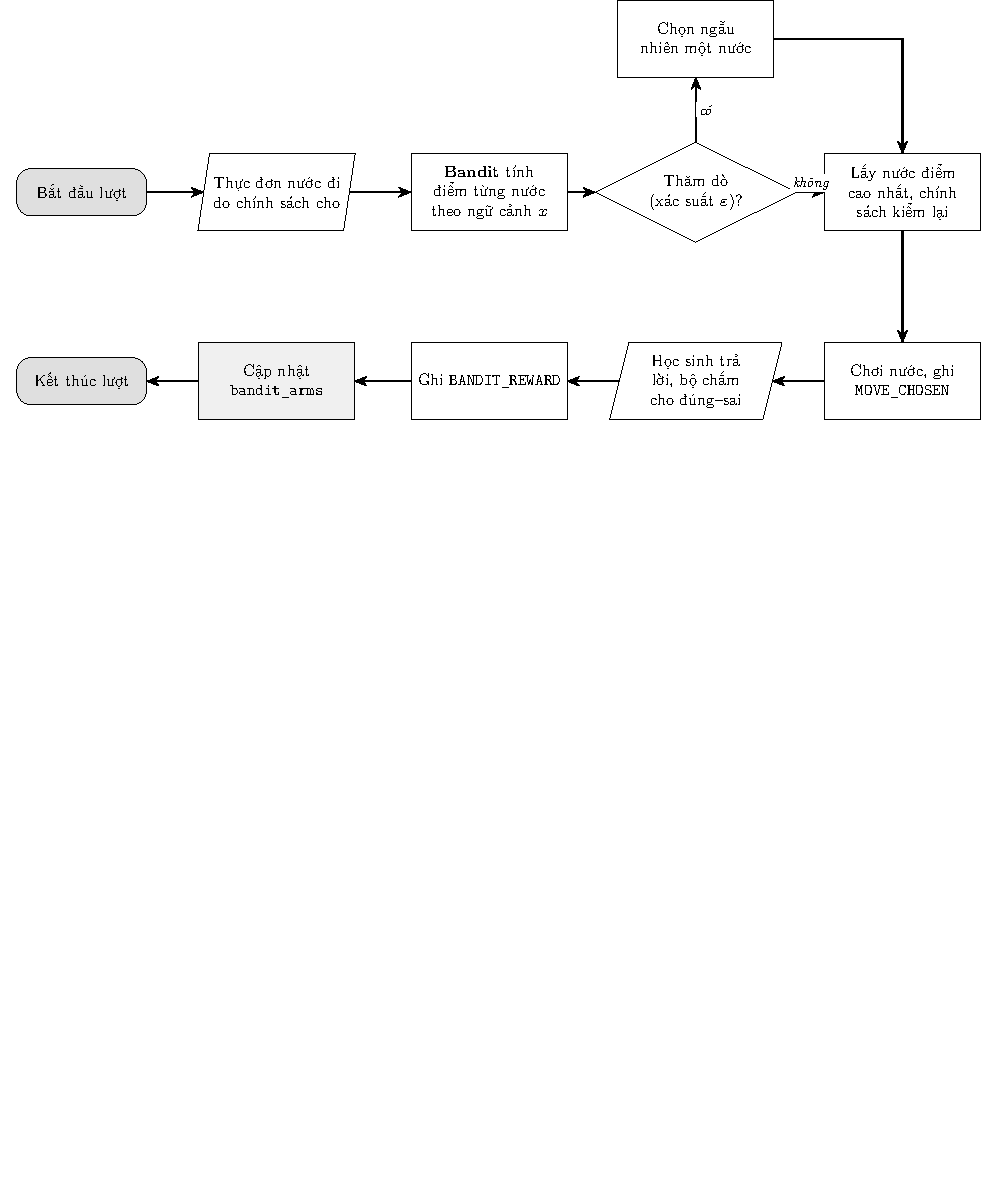
\includegraphics[width=\linewidth]{figures/pdf/fig-bandit-flow.pdf}
\caption{Vòng chọn nước đi và vòng học của bandit trong một lượt. Hàng trên là lượt chọn; hàng dưới là cách câu trả lời kế tiếp của học sinh trở thành phần thưởng và cập nhật kho trạng thái.}
\label{fig:bandit-flow}
\end{figure}

Cánh tay là loại nước đi cùng bậc của nó, chẳng hạn hỏi lại cách làm, gợi ý ở bậc hai hay đưa phản ví dụ, nên một cánh tay mang cùng nghĩa trên mọi thực đơn. Nước đóng câu hoặc xác nhận để sang câu sau không phải cánh tay của bandit; thực đơn có nước như vậy được chuyển cho bộ chọn dự phòng. Ngữ cảnh là chín số trong $[0,1]$ rút từ tình hình của học sinh trên câu đang làm: hằng số chặn, số lần trả lời, số gợi ý đã nhận, bậc gợi ý cao nhất, số lượt chưa tiến bộ, số lần xin gợi ý, dấu hiệu nản, việc gia sư đã hỏi cách làm chưa và số lần lặp lại của lỗi quan niệm hay gặp nhất, mỗi số được chặn rồi chia về $[0,1]$. Ngữ cảnh chỉ gồm số đếm, không chứa phản hồi học sinh hay đáp án, nên bandit không thể làm lộ đáp án.

Phần thưởng của một lượt chọn là giá trị của câu trả lời có chấm kế tiếp trên cùng câu, trừ chi phí theo mức giúp, theo công thức~\eqref{eq:reward} ở Chương~\ref{chap:theory}: một câu hỏi lại đưa học sinh tới câu đúng được đúng $1$, còn gợi ý bậc một đưa tới câu đúng được $1-0{,}3/7\approx0{,}96$. Lượt chọn không có câu trả lời có chấm theo sau, vì câu đóng trước, hoặc bị chính sách từ chối thì không được trả thưởng. Mỗi cánh tay nhận điểm cận trên tin cậy theo công thức~\eqref{eq:linucb} với $\alpha=0{,}5$ và ridge bằng $1$. Bộ chọn lấy cánh tay điểm cao nhất với xác suất $0{,}9$ và chọn đều với xác suất $0{,}1$; hai cánh tay hòa điểm thì nước của chính sách thắng, nên bandit chưa học gì chơi đúng nước chính sách sẽ chơi. Số ngẫu nhiên sinh từ mã băm của khóa phiên, số lượt và đề bài, nên cùng phiên, lượt và thực đơn luôn cho cùng lựa chọn.

Mỗi lượt chọn được ghi vào nhật ký cùng cánh tay, xác suất của lượt chọn, vector ngữ cảnh và điểm của mọi cánh tay trong thực đơn, còn sự kiện phần thưởng ghi cánh tay, ngữ cảnh, phần thưởng và phiên bản bandit. Trạng thái học gồm ba đại lượng cộng được cho mỗi cánh tay: $\sum xx^{\top}$, $\sum rx$ và số lượt. Tính cộng được có hai hệ quả: thứ tự phần thưởng không ảnh hưởng tới trạng thái, và mỗi phần thưởng là một phép cộng nguyên tử vào một tài liệu, phù hợp cơ sở dữ liệu không có giao dịch nhiều tài liệu. Cập nhật diễn ra sau khi lệnh của học sinh được ghi thành công nên lệnh lặp không trả thưởng hai lần, và toàn bộ kho dựng lại được từ các sự kiện phần thưởng. Mô hình ngôn ngữ không ghi vào kho này. Tham số \texttt{TUTOR\_CHOOSER=bandit} bật bộ chọn; mặc định vẫn là bộ chọn bằng mô hình cho tới khi chủ dự án duyệt tham số của bandit. Bandit giữ nguyên sáu bất biến của đồ án.

\section{Mở rộng sang Tiếng Anh và giọng nói}\label{sec:english-design}
Môn Tiếng Anh được thêm vào sau khi gia sư Toán đã được đo và duyệt, nên yêu cầu thiết kế quan trọng nhất là không làm đổi hành vi, công thức, ngưỡng, lời nhắc hay kết quả đánh giá của Toán và không để nội dung hai môn lẫn vào nhau. Hệ thống giữ điều này bằng cách đặt môn học thành thuộc tính bắt buộc ở mọi tầng thay vì cờ ở giao diện. Mọi tài liệu giáo viên, câu trong ngân hàng, gói bài và gói chương mang trường môn học, và thiếu trường này là lỗi kiểm tra dữ liệu. Bộ đọc tài liệu Tiếng Anh là mô-đun riêng được chọn theo môn của tài liệu mà không sửa nhánh xử lý của Toán. Mỗi môn có chỉ mục truy xuất dựng riêng từ đầu và bộ tách từ riêng, thay vì một chỉ mục chung rồi lọc lúc truy xuất. Môn của một buổi được ghi vào chính tài liệu buổi khi tạo, nên buổi cũ luôn được hiểu đúng môn. Các phần dùng chung, như phép chiếu mức hiểu, chính sách trên đồ thị, vòng dạy và cổng AI, chỉ được thêm một nhánh theo môn đọc từ gói nội dung của buổi, không tham số nào do máy khách chọn. Kiểm tra dữ liệu từ chối gói thiếu môn, kiểm tra dựng chỉ mục chứng minh chỉ mục hai môn không chứa đoạn của nhau, và bộ kiểm tra chuẩn của Toán được chạy lại trước mỗi thay đổi chạm phần dùng chung với yêu cầu kết quả giống hệt.

Phạm vi Tiếng Anh là Unit~11 ``Family time'' của lớp 5, gồm sáu bài về hỏi đáp chuyện đã xảy ra bằng thì quá khứ đơn (``Did you\ldots''), từ vựng về một chuyến đi và một đoạn đọc ngắn. Gia sư ôn bài theo cùng vòng sáu bước và cùng phép chiếu mức hiểu; cô giảng bằng tiếng Việt, còn câu đích học sinh nói hay chọn là tiếng Anh. Đáp án và câu hỏi chỉ lấy từ tài liệu chủ dự án cung cấp, và không mô hình nào được tạo đáp án cho câu kiểm tra. Bộ chấm nhận nhiều biến thể hợp lệ, phân biệt lỗi chính tả với lỗi ngữ pháp, coi một từ đúng là đúng một phần và nhận câu trả lời bằng tiếng Việt. Chính sách mức hiểu riêng có ba khác biệt: một lớp lỗi về ảnh hưởng của tiếng mẹ đẻ, câu nói theo cô được tính độc lập tối đa như bậc H6, và độ tin cậy nhận dạng giọng nói được đưa vào bằng chứng.

Chế độ giọng nói cho phép học sinh nhập bằng tiếng nói thay vì văn bản. Dịch vụ nhận dạng của Groq trả bản chép lời kèm độ tin cậy, còn lời gia sư được phát bằng giọng tổng hợp chạy trên máy của người vận hành. Bản chép lời độ tin cậy thấp không được coi là câu trả lời chắc chắn: độ tin cậy đi vào trọng số bằng chứng và lượt nhận dạng kém được lưu để giáo viên nghe lại. Giọng nói chỉ là phương thức nhập và xuất, không phải thành phần quyết định: sau nhận dạng, phản hồi đi qua cùng quy trình như văn bản nên mọi bất biến ở mục~\ref{sec:nfr} giữ nguyên.

\section{Dữ liệu, tài khoản, triển khai và chi phí vận hành}\label{sec:data-design}
Dữ liệu cốt lõi là một sổ sự kiện chỉ ghi thêm cho mỗi buổi học. Mỗi sự kiện có kiểu, nội dung, thời điểm, số thứ tự trong buổi và mã trường; các kiểu gồm phản hồi học sinh, lời gia sư, quyết định chính sách, câu hiển thị, câu trả lời đã chấm, gợi ý, câu được khép, lệnh gọi và chuyển mô hình, phản hồi bị từ chối và phần thưởng bandit. Chính sách, điểm hiểu bài và mọi báo cáo là phép chiếu tất định từ sổ này, nên phát lại một buổi không cần gọi lại mô hình: lựa chọn của mô hình đã nằm trong sổ. Cơ sở dữ liệu là MongoDB Atlas gói miễn phí M0, không hỗ trợ giao dịch nhiều tài liệu, nên trạng thái và sự kiện của một buổi nằm trong một tài liệu ghi nguyên tử với số phiên bản để phát hiện hai lần ghi chồng nhau. Tệp gốc và âm thanh nằm trên ổ đĩa máy chủ. Database phát triển, kiểm thử và dữ liệu thật được tách tuyệt đối: kiểm thử chạm cơ sở dữ liệu thật chỉ chạy trên database tạm có tên theo mẫu cho phép và tự dọn, dữ liệu demo chỉ tạo bằng một lệnh riêng và gắn cờ để xóa được, và không script nào tự ghi vào database phát triển hay thật.

Giáo viên đăng nhập bằng mã PIN lưu dạng băm một chiều. Học sinh tự tạo tài khoản bằng tên đăng nhập và mã bí mật bốn đến tám chữ số. Phụ huynh dùng chung tài khoản của con và nhận mã vai trò riêng nên chỉ xem được báo cáo của con. Máy chủ ký mã xác thực bằng khóa riêng của lần triển khai, mọi ràng buộc quyền được thực thi ở máy chủ theo vai trò, và máy khách không có đường nào chọn mô hình hay vượt ràng buộc của buổi học.

Khi phát triển, hệ thống chạy trực tiếp trên máy không dùng Docker, một cổng phục vụ cả web và API. Khi lên máy chủ, người vận hành dùng Docker Compose với một ảnh chứa web và API cùng một MongoDB riêng có mật khẩu và không mở cổng ra ngoài. Dữ liệu database nạp từ tệp xuất bằng lệnh chỉ đọc; vì kho mã công khai và tệp chứa lời các em đã nói, tệp này không bao giờ nằm trong kho mà đi qua kênh riêng. Bộ kiểm thử chạy hoàn toàn ngoại tuyến, không cần mạng hay database thật.

Về chi phí và khả năng mở rộng, hệ thống chạy hoàn toàn trên dịch vụ miễn phí nên chi phí tiền bằng không, nhưng hạn mức là giới hạn thật. Mỗi lượt gọi mô hình vài lần, mỗi lần tốn trung bình khoảng $1\,100$ token và lời nhắc không quá $3\,000$ token, nên hạn mức khoảng $8\,000$ token mỗi phút giới hạn số học sinh học đồng thời ở mức vài em trên một khóa; trần số lệnh gọi theo buổi và theo chương giữ cho một buổi không dùng hết hạn mức của người khác, và câu mẫu đảm bảo buổi học không dừng khi hạn mức cạn. Đồ án chưa đo độ trễ từng lượt và chưa kiểm chứng việc phục vụ nhiều học sinh cùng lúc; việc mở rộng đòi chuyển sang gói trả phí hoặc mô hình chạy cục bộ, và đây là một hạn chế được nêu ở mục Kết luận.

\section{Tổng kết chương}
Chương này trình bày thiết kế trong đó hệ thống học tập được dựng trước và mô hình ngôn ngữ chỉ giữ vai diễn đạt. Sáu bất biến ở mục~\ref{sec:nfr} được giữ bằng các thành phần tất định: vòng sáu bước và thang gợi ý quyết định điều gia sư làm, truy xuất lai theo đồ thị giới hạn điều gia sư được dạy, bộ chấm và phép chiếu mức hiểu quyết định điều học sinh đã làm được, và bộ kiểm chứng chặn lời của mô hình khi vi phạm. Bộ chọn bandit (mục~\ref{sec:bandit-design}) là phần học được duy nhất và vẫn nằm trong thực đơn mà chính sách cho phép. Chương sau đánh giá các thành phần này.

